\documentclass[9pt,twocolumn,twoside,lineno]{pnas-new}
% Use the lineno option to display guide line numbers if required.

\templatetype{pnasresearcharticle} % Choose template 
% {pnasresearcharticle} = Template for a two-column research article
% {pnasmathematics} %= Template for a one-column mathematics article
% {pnasinvited} %= Template for a PNAS invited submission

\title{The Exception, Not the Rule: Sandy Hook and Firearm Purchases}

% Use letters for affiliations, numbers to show equal authorship (if applicable) and to indicate the corresponding author
\author[a,1]{David Liu}
\author[b,1]{Sri Nimmagadda} 

\affil[a]{Princeton University, Department of Computer Science}
\affil[b]{Princeton University, Woodrow Wilson School of Public and International Affairs}

% Please give the surname of the lead author for the running footer
\leadauthor{Liu} 

% Please add here a significance statement to explain the relevance of your work
\significancestatement{Authors must submit a 120-word maximum statement about the significance of their research paper written at a level understandable to an undergraduate educated scientist outside their field of speciality. The primary goal of the Significance Statement is to explain the relevance of the work in broad context to a broad readership. The Significance Statement appears in the paper itself and is required for all research papers.}

% Please include corresponding author, author contribution and author declaration information
\authorcontributions{Please provide details of author contributions here.}
\authordeclaration{Please declare any conflict of interest here.}
\equalauthors{\textsuperscript{1}A.O.(Author One) and A.T. (Author Two) contributed equally to this work (remove if not applicable).}
\correspondingauthor{\textsuperscript{2}To whom correspondence should be addressed. E-mail: author.two\@email.com}

% Keywords are not mandatory, but authors are strongly encouraged to provide them. If provided, please include two to five keywords, separated by the pipe symbol, e.g:
\keywords{Mass Shootings | Sandy Hook | Gun Sales | National Rifle Association} 

\begin{abstract}
As mass shootings continue to arise in the United States, it is important to understand the public's response to these shootings. While previous studies have focused on the large number of gun sales following the Sandy Hood and San Bernardino shootings, we take a more comprehensive analysis. Our findings show that prior to Sandy Hook, shootings did not foreshadow an increase in gun sales, even for deadly shootings like the Fort Hood shooting in 2009. Instead, Sandy Hook was a turning point. We follow with suggestive findings that the threat of gun control legislation instigated the the spike in gun sales following Sandy Hook The same political climate enabled a rise in gun sales following the San Bernardino shooting at the end of the Obama presidency. On the other hand, though equally, if not more tragic, the recent Parkland shooting did not precede a peak in gun sales with the Trump administration stifling the possibility of gun control. Our findings suggest that the mere attempt to pass gun control legislation, irrespective of its success, may cause a short term increase in gun sales. 
\end{abstract}

\dates{This manuscript was compiled on \today}
\doi{\url{www.pnas.org/cgi/doi/10.1073/pnas.XXXXXXXXXX}}

\begin{document}

\maketitle
\thispagestyle{firststyle}
\ifthenelse{\boolean{shortarticle}}{\ifthenelse{\boolean{singlecolumn}}{\abscontentformatted}{\abscontent}}{}

% If your first paragraph (i.e. with the \dropcap) contains a list environment (quote, quotation, theorem, definition, enumerate, itemize...), the line after the list may have some extra indentation. If this is the case, add \parshape=0 to the end of the list environment.
\dropcap{I}t is an often-stated political trope that mass shootings, counter-intuitively, increase gun sales as opposed to diminish them due to fear from gun-owners regarding the passage of gun-control measure\cite{pinsker_why_2017}. The political aftermath of the Sandy Hook shooting serves as a valuable case study in this regard. On December 12th, 2012, a shooter entered the Sandy Hook Elementary School campus and opened fire, killing 26 – most of whom were children at the school. Previous research has demonstrated that Obama’s call to action after this event and specific proposals to restrict access to guns contributed to a large increase in gun exposure, which in turn led to an increase in accidental deaths[2]. The implication of this study is two-fold: For one, it confirms the relationship between increases in gun exposure and the accidental firings of firearms. However, this study also appears to corroborate the notion that the political implications of mass shootings have identifiable effects on the sale of firearms.

However, Levine and McKnight's 2017 study 'Firearms and accidental deaths: Evidence from the Sandy Hook school shooting" aligns state-level background check data solely against the Sandy Hook school shooting, with little to no evidence regarding any other shooting that occurred during the same period. This method assumes that the findings in the case of the Sandy Hook shooting are generalizable to all contemporary mass shootings that have occurred in the United States. Upon further inspection, it's possible that this is not the case - different mass shootings can have occurred in different time periods and political contexts, thereby affecting their political ramifications on the likelihood of gun legislation and firearm sales. Identifying differences and similarities in the effects of mass shootings on firearm sales can be valuable towards understanding the political and psychological drivers of firearm sales in the United States.

Consider, for example, the San Bernardino shooting and the Parkland shooting at Marjory Stoneman High School. The Parkland shooting's death count actually exceeded that of the San Benardino shooting's death count; however, background checks for firearm sales declined after the Parkland shooting and increased after the San Benardino shooting. Conventional explanations for why certain tragedies gain political traction as opposed to others fails to account for this difference, as one may expect the firearm sales after the Parkland shooting to exceed sales after the San Benardino shooting due to the location of the attack in a school lending emotional credence to the gun control movement. Yet this isn't the case, forcing us to question why some shootings have positive effects on firearm sales whereas others have negative effects. 

As such, this study is primarily concerned with identifying the effects of mass shootings on gun exposure throughout the United States by looking at the largest mass shootings by casualty count over the past fifteen years to identify either similarities or differences in resultant changes in firearm sales post-shooting. In order to do so, we employ similar methods to Levine and McKnight in that we visualize background check data with respect to the various large mass shootings that have occurred in the United States over the past fifteen years. We extend this study by placing this time-series background check data - used as a variable to measure gun exposure - at the state and national level in the context of the states and geographic regions within which they occur. 

By conducting this exercise, we identify differences in firearm sales effects at the local and national level between shootings. As a result, we find that Sandy Hook was actually the exception - not the rule - in its positive influence on firearm sales at both the local and national levels whereas other shootings - including the Geneva County shooting, the Fort Hood shooting, and the San Benardino massacure - have actually been followed by periods of depressed firearm sales. In our discussion, we consider the political ramifications of this finding and suggest methods and future studies that can better identify the causal mechanisms through which mass shootings affect gun sales. 
%------------------------------------------------
\section{Materials and Methods}
To compare the number of gun sales after multiple mass shootings, we collected background check data, as reported by the FBI, and then normalized with the National Cancer Institute's population data. To complete the data cleaning, we detrended the normalized data with month and year fixed effects. Finally, we used Google Trends data to measure the public's interest and awareness of gun control legislation. 
\subsection{Origin of Background Check Data}

We collected state-level monthly background check counts from the FBI’s National Instant Background Check System (NICS) \footnote{https://www.fbi.gov/file-repository/nics\_firearm\_checks\_-\_month\_year\_by\_state.pdf/view}. The data spanned all fifty states and every month between 2007 - 2016, inclusive. A background check is completed every time an individual attempts to purchase a firearm from a Federal Firearm Licensee  (FFL). Because a check is performed prior to every purchase, the quantity of NICS background checks serves as a proxy for the number of firearms sold \cite{PBL}. 
	Furthermore, the NICS data is well suited for comparing background check counts between states because all states must comply with the system under the 1993 Brady Act, a piece of federal legislation. In this regard, even though gun control legislation varies state by state, federal law standardizes the record of background checks, creating a single system by which states report the number of checks. 
	To prepare for intrastate comparisons, we normalized the background checks by population. These annual population data were reported by the National Cancer Institute’s Surveillance, Epidemiology, and End Result Program (SEER). The raw population data  from NCI breaks the population down by race and county, so to state-level analysis, we grouped the data by state. These aggregated state population counts matched previous aggregations of the NCI data \cite{levine_firearms_2017}. With the aggregated data, we were able to calculate the number of background checks that occured in a given month per 100,000 individuals. 
    A brief analysis of the normalized background check data shows that the number of background checks as well as the variance from month to month varies widely among states. Figure \ref{fig:boxplot} shows boxplots of population-normalized background checks counts in the months between 2007 and 2016. On one hand, we have states like New Jersey which only average 70 background checks, with little variation between months. On the other hand, we have states like Alabama, which averages over 700 normalized background checks per month. At the same time, at its peak, the number of background checks in Alabama reaches has high as 2500. The takeaway is that some states experiences higher variation in background check counts. 
\begin{figure}%[tbhp]
  \centering
  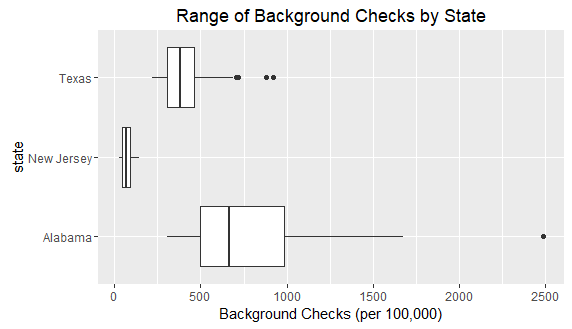
\includegraphics[width=\linewidth]{figures/boxplot}
  \caption{Of the states we analyzed, the average number of normalized background checks counts ranged from as high as 775 in Alabama to as low as 70 in New Jersey.}
  \label{fig:boxplot}
\end{figure}
	It is important to note that while the NICS data can be used as a proxy for firearms sales, they are not precise estimates. In fact, background checks are not required for intrastate transfers between private parties. Furthermore, firearms are purchased through unlicensed dealers, who to not earn a living from selling firearms. Many of these unlicensed purchases are made at local gun shows and do not lead to background checks. A recent 2017 survey found that at least 22\% of firearms are purchased through unlicensed sellers \cite{miller_firearm_2017}. So, the number of background checks reported by NICS is a lower bound on the actual number of guns sold.
    
\subsection{Detrending Firearm Seasonal Trends}

It is known that firearms purchases vary by season and year. Each year, more firearms are sold in the winter than the summer. At the same time, firearms sales have been steadily increasing over the past decade. In order to analyze variation in firearms sales and compare sales at multiple points in time, it is necessary to detrend the data. 
	To detrend the data, we applied month and year fixed effects. The two sets of fixed effects capture our prior knowledge of seasonal patterns in firearms sales. Because these seasonal trends may vary from state to state, we composed a fixed effects model for each state. For a given month, year, and state, we decompose the number of background checks as such:
\begin{figure}
\begin{align}
(x+y)^3&=(x+y)(x+y)^2\\
       &=(x+y)(x^2+2xy+y^2) \numberthis \label{eqn:example} \\
       &=x^3+3x^2y+3xy^3+x^3. 
\end{align}    
\end{figure}
Henceforth, our metric for the number of background checks will be the residual from the above decomposition. This value captures the amount of deviation from the seasonal trend and can be interpreted as the number of background checks relative to the expected quantity based on temporal trends. When the residuals are positive, the quantity expresses the number of additional background checks in a given month. 

\subsection{Coefficient Analysis}

To confirm that our fixed effects model performed as expected based on prior firearms domain knowledge, we visualized the coefficients from the model, as shown in Figure x. While we composed a fixed effects model for each state to detrend the data, the overall patterns shown below reflect national trends. 
\begin{figure}%[tbhp]
  \centering
  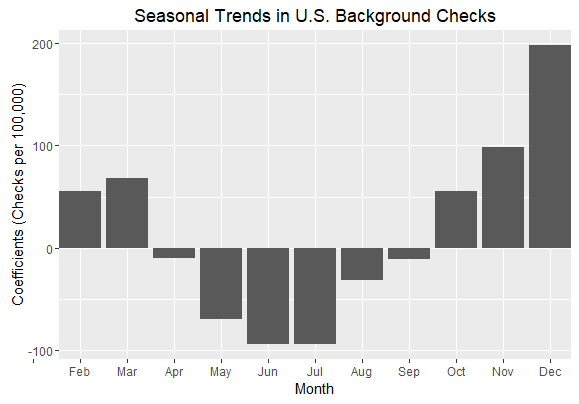
\includegraphics[width=\linewidth]{figures/seasonal}
  \caption{Placeholder image of a frog with a long example caption to show justification setting.}
  \label{fig:monthly}
\end{figure}
	In the seasonal plot, the baseline value is the month and January, and in the yearly plot, the baseline year is 2007. From the monthly plot, we can see that firearms sales do peak in the winter (December) and trough in the summer (June and July). Between the peak and the trough there is a difference of 300 background checks per 100,000 individuals.
\begin{figure}%[tbhp]
  \centering
  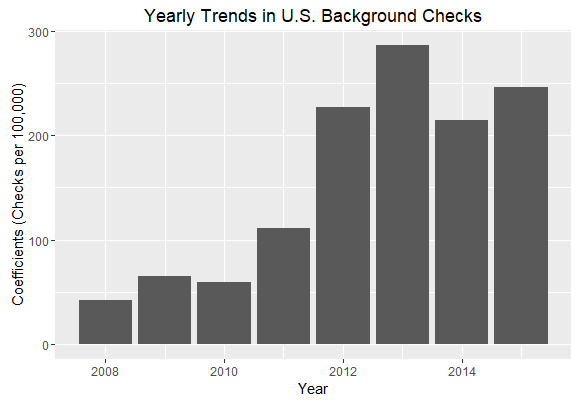
\includegraphics[width=\linewidth]{figures/yearly}
  \caption{Placeholder image of a frog with a long example caption to show justification setting.}
  \label{fig:monthly}
\end{figure}  
    And then, from the yearly plot, we can see that firearm sales have been increasing since 2007, especially in 2012 and 2013. The order of magnitude in the yearly coefficients is similar to the monthly ones. 
    
\subsection{Comparable Deadly Shootings}

	To study the response in firearm sales to mass shootings beyond Sandy Hook and San Bernardino, we compiled a list of the remaining deadliest shootings in the 2007 - 2016 period. These shootings include the Orlando nightclub, Virginia Tech, Binghamton, and Fort Hood, and Geneva County Massacres. These shootings killed 50, 33, 14, 14, and 11 people respectively. Because all of these shootings ranked in the top 20 deadliest shootings in US history, we were able to control for the role of death toll in the subsequent effect on gun sale purchases. 
	Of note, the Aurora and Washington Navy Yard shootings were not included, though they were deadly enough, because of the proximity to the Sandy Hook shootings. 
    
\subsection*{Gun Control Analysis}

For our analysis, we needed a measure of the public’s belief in the feasibility of gun control. This is independent from the public’s opinion on gun control itself; instead, we were curious in the public’s views on the chances of gun control legislation passing. The feasibility of gun control has been the topic of Pew surveys in the past. However, these surveys were far and few between for our purposes. To analyze background checks and gun control prospects simultaneously, we sought monthly estimates of gun control likelihoods. 
	Turning to a big-data source, we utilized Google Search Trends. We collected data on searches for “gun control” in the United States from 2007 - 2018, where the values are scaled relative to the maximum value. As used in previous works, the Google Search trends can be interpreted as the public’s interest in a particular topic at given moment in time. Conveniently, the trends data are also stored in monthly intervals. 
%------------------------------------------------

\section{Results}
\begin{figure*}%[tbhp]
\centering
\begin{subfigure}{.5\textwidth}
  \centering
  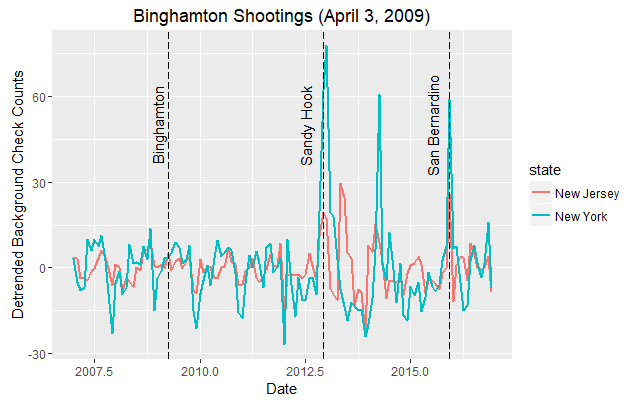
\includegraphics[width=\linewidth]{figures/binghamton}
\end{subfigure}%
\begin{subfigure}{.5\textwidth}
  \centering
  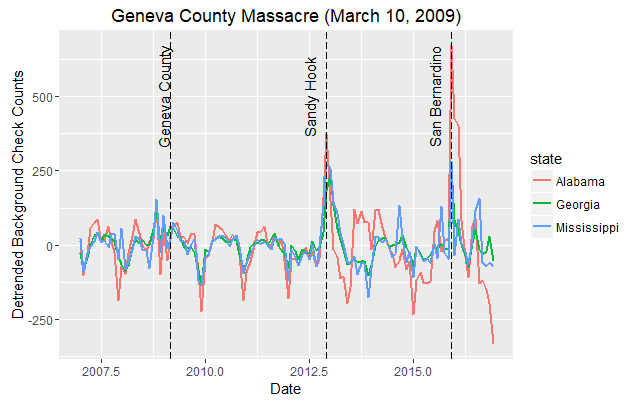
\includegraphics[width=\linewidth]{figures/geneva-county}
\end{subfigure}
\caption{Placeholder image of a frog with a long example caption to show justification setting.}
\label{fig:}
\end{figure*}

\subsection{Shootings During Obama's First Term Did Not Precede Increases in Background Checks}

Figures x, x, and x all show detrended background check quantities following each of the shootings that preceded Sandy Hook. In each of the figures, only the states in the proximity of the shooting in question are shown. These states were chosen with the hypothesis that a change in background checks would be most likely near the site the shooting itself. For example, it has been shown that individuals purchases guns following a mass shooting for the purpose of self-protection. It is then reasonable to hypothesize that those living near the scene of a shooting would be moved to purchase a firearm. 
\begin{figure}
  \centering
  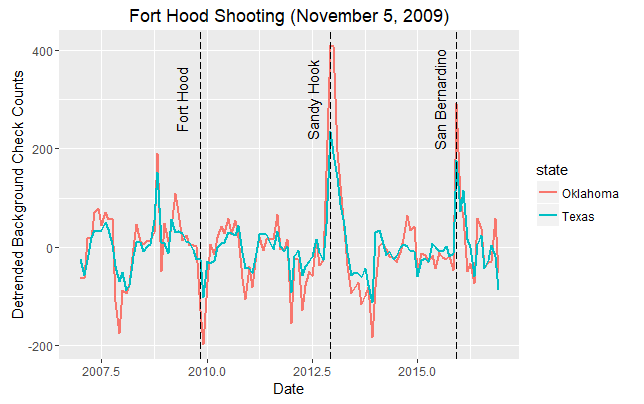
\includegraphics[width=\linewidth]{figures/fort-hood}
  \caption{Placeholder image of a frog with a long example caption to show justification setting.}
  \label{fig:fort-hood}
\end{figure}
Nonetheless, the three figures show that even in the host states, gun sales did not increase following 2009 era shootings. In the case of the Binghamton and Geneva shootings, there is no noticeable change in background check levels. Following the Fort Hood shootings, background checks appear to dip in Texas and Oklahoma, but this is likely an artifact of the Sandy Hook and San Bernardino shootings on the fixed effects; because both of the later shootings took place in December, the December coefficient in the fixed effects model is likely inflated. For comparison, the dip in background checks following the Fort Hood shootings is similar in magnitude to the dip at the end of 2007, suggesting background checks varied similar to years past despite the mass shooting. 

\subsection{Sandy Hook Increased Background Checks Nationally}

In contrast, background checks increased precipitously in all of the states shown following the Sandy Hook and San Bernardino shootings. In New York, the deviation in background checks was five times larger than any previous deviation, and in Oklahoma, the peak following Sandy Hook was two times higher than any previous peak. The key takeaway is that even in states far and distant from the site of the original shootings, Connecticut and California, background checks increased following the Sandy Hook and San Bernardino shootings. 

It is also helpful to note that the response to the shootings occurred immediately and lasted for a short duration. The Sandy Hook shooting took place on December 14, 2012 and by January 2013, we already see a peak in background checks. Similarly, the San Bernardino attack took place on December 2, 2015 and background checks spike in that same month. In fact, for both of the shootings, background checks had fallen back to expected levels in just two months after the events. So, the response in gun sales to the Sandy Hook and San Bernardino shootings was quick, widespread, and pronounced but also short lasted. 
\subsection{Attempts to Institute Gun Control Correlated Positively with Background Checks}

Because the response to the Sandy Hook shooting was unprecedented, it is natural to ask what factors led to the pronounced spike in background checks. One possible hypothesis is that the aftermath of the Sandy Hook shooting also coincided with the first serious attempt to pass gun control legislation under the Obama administration. Previously, especially in the earlier half of Obama’s first term, the possibility of gun control was not serious even after the series of shootings in 2009. Following, Sandy Hook, however, the political climate was different. Obama had already been re-elected, clearing the path for a renewed effort to pass gun control. In fact, just five days after the Sandy Hook shooting, Obama broke ground on the path towards gun control by calling Congress to ban assault rifles and initiating a working group to make recommendations for gun control. 
\begin{figure}
  \centering
  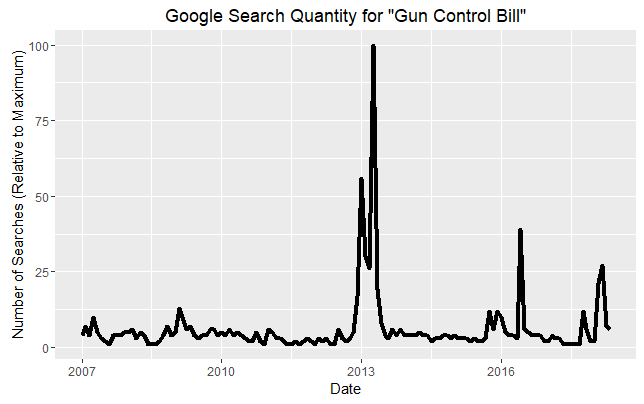
\includegraphics[width=\linewidth]{figures/google-trends-gun-control}
  \caption{Placeholder image of a frog with a long example caption to show justification setting.}
  \label{fig:gtrends}
\end{figure}
	Our own data from Google Trends suggests that Obama’s renewed attempts to pass gun control were noticed by the general public. Figure x shows that searches for “Gun Control Bill” skyrocketed after the Sandy Hook shooting. In fact, Google Searches for gun control in the month following Sandy Hook were eight times larger than any month in the previous five years. These results suggest that public interest and awareness of gun control were also unprecedented following Sandy Hook. 
    
	The correlation between a spike in gun sales and pushes for control persists for the San Bernardino attacks, which took place the end of the Obama’so second term. In the Google Trends, we can see a second pronounced wave of interest in gun control. The spike was less than half the spike in searches following Sandy Hook but still the second highest spike in in the nine year period between 2007 - 2015. So in both the cases of Sandy Hook and San Bernardino, we observe unprecedented spikes in background checks but also public awareness of gun control. 

\subsection{Spikes in Background Checks After Mass Shootings Were Muted During a Trump Presidency}

To put the hypothesis that the possibility of gun control and background checks are correlated, we can analyze the much more recent shooting at Stoneman Douglas high school in Parkland, Florida. Very similar to Sandy Hook, this shooting took the lives of young children while also capturing the nation’s attention. However, unlike Sandy Hook and San Bernardino, the Parkland shooting took place under the Trump presidency and a Republican controlled congress, with few prospects for gun control legislation. 
\begin{table}[!htbp] \centering 
	\caption{Linear model of Florida's Population 2007 - 2016} 
	\label{} 
	\begin{tabular}{@{\extracolsep{5pt}}lc} 
		\\[-1.8ex]\hline 
		\hline \\[-1.8ex] 
		& \multicolumn{1}{c}{\textit{Dependent variable:}} \\ 
		\cline{2-2} 
		\\[-1.8ex] & pop \\ 
		\hline \\[-1.8ex] 
		year & 249,418.100$^{***}$ \\ 
		& (12,878.980) \\ 
		& \\ 
		Constant & $-$482,380,604.000$^{***}$ \\ 
		& (25,906,085.000) \\ 
		& \\ 
		\hline \\[-1.8ex] 
		Observations & 10 \\ 
		R$^{2}$ & 0.979 \\ 
		Adjusted R$^{2}$ & 0.977 \\ 
		Residual Std. Error & 116,979.100 (df = 8) \\ 
		F Statistic & 375.054$^{***}$ (df = 1; 8) \\ 
		\hline 
		\hline \\[-1.8ex] 
		\textit{Note:}  & \multicolumn{1}{r}{$^{*}$p$<$0.1; $^{**}$p$<$0.05; $^{***}$p$<$0.01} \\ 
	\end{tabular} 
\end{table} 
\begin{figure}
  \centering
  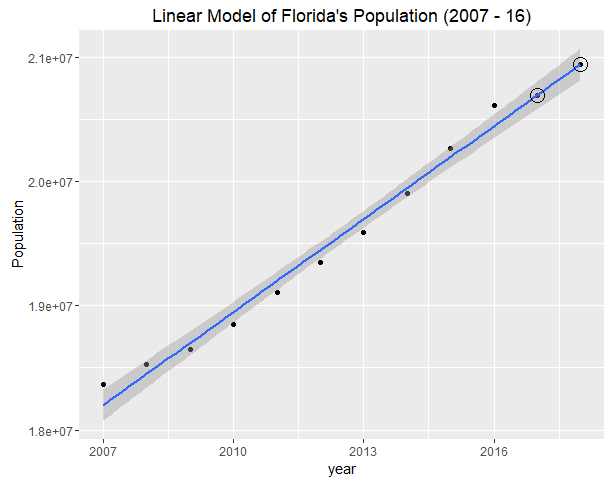
\includegraphics[width=\linewidth]{figures/florida}
  \caption{Placeholder image of a frog with a long example caption to show justification setting.}
  \label{fig:florida}
\end{figure}
	In order to apply our methodology to the Parkland shooting, we needed to estimate Florida’s population in 2017 and 2018 because the latest SEER population data extends only up until 2016. Fortunately, between 2007 and 2016, Florida’s population followed an extremely linear trajectory. In fact, a linear regression on Florida’s population over the decade has an R-squared of 0.979, with the population rising by a quarter million each year. With this linear model, we made predictions of Florida’s population in 2017 and 2018. On the other hand, we did have access to up-to-date background checks from the NICS. 
	After detrending the background check levels, we produced the graph shown in Figure x. The graphs shows background check counts in Florida between 2007 and 2018, which spans the Sandy Hook, San Bernardino, and Parkland shootings. The figure shows that after Sandy Hook and San Bernardino, monthly background check levels were approximately 200 counts / 100,000 higher than expected. In contrast, background checks following the Parkland shooting were only 100 counts / 100,000 higher than anticipated, a peak half in magnitude compared to the shootings that took place during Obama’s second term. Our analysis of the previous shootings demonstrated that any peak in background checks following a mass shooting occurred quickly, within a month of the date of the shooting. The Parkland data shows a peak in background checks for the month of March but by April, background checks had already fallen to expected levels. So, we do not expect any further spike in background checks following the Parkland shooting. 

The diminished peak in background checks following the Parkland shootings relative to the Sandy Hook and San Bernardino shootings supports our hypothesis that the threat of gun control explains the unprecedented backlash during the Obama administration. Under Trump, the possibility of gun control has decreased, even after a mass shooting. Our Google Trends results show that searches for a gun control bill following Parkland were a quarter of the level they reached after Sandy Hook. Taken together these observations undermine the hypothesis that the traumatic nature of the Sandy Hook and San Bernardino caused an increase in background checks for the Parkland shooting also captured national attention. Instead,  the decreased possibility for gun control under president Trump has diminished the imminent threat of legislation to gun owners after mass shootings. 

%------------------------------------------------

\section{Discussion}

As we've found, there appears to be a difference in the effects of different shootings on firearm sales at both the local and national levels between different events, proving that Sandy Hook was the exception - \textit{not the rule} - in its effects on gun exposure. This finding appears to corroborate the notion that the occurrence of mass shootings in and of themselves is not enough to influence firearms sales in one direction or another. In fact, the political context within which shootings occur matters. 

This finding is significant for a multitude of reasons, some political and some methodological. For one, this finding complicates the popular trope mentioned at the beginning of this study in that mass shootings do not uniformly increase gun exposure. However, our analysis primarily depends on the alignment of time-series background check data with their contemporary political events, which is hardly proof of definite causation. So, how can we prove the causal mechanisms that connect mass shootings to firearm sales?

INSERT DAG HERE

Based on the dag above, we assume that mass shootings influence public perception regarding firearms and the likelihood of gun control, likely through the CNN effect - a term coined to describe the effect that major news media outlets have on the political and economic climate of the United States by amplifying certain news stories and events. Therefore, we can see that mass shootings may influence media coverage, which in turn may influence domestic policy. But under the top-down model of domestic politics, one could find that the media responds to elite cues set forth by the Presidency or government to advance certain foreign policy ideas or agendas. With this in mind, it's entirely possible that factors endemic to an administration and independent of a shooting could affect public perception of firearms and, in turn, public perception of the likelihood of gun control passing at the state or even national levels. 
\acknow{Please include your acknowledgments here, set in a single paragraph. Please do not include any acknowledgments in the Supporting Information, or anywhere else in the manuscript.}

\showacknow{} % Display the acknowledgments section

% Bibliography
\bibliography{pnas-sample}

\end{document}